\documentclass{article}
\usepackage{listings}
\usepackage{mathrsfs}
\usepackage[utf8]{inputenc}
\usepackage{amssymb}
\usepackage{lipsum}
\usepackage{amsmath}
\usepackage{fancyhdr}
\usepackage{geometry}
\usepackage{scrextend}
\usepackage[english,german]{babel}
\usepackage{titling}
\setlength{\droptitle}{-3cm}
\usepackage{tikz}
\usepackage{algorithm,algpseudocode}
\usepackage[doublespacing]{setspace}
\usetikzlibrary{datavisualization}
\usetikzlibrary{datavisualization.formats.functions}
\usepackage{polynom}
\usepackage{amsmath}
\usepackage{gauss}
\usepackage{tkz-euclide}
\usetikzlibrary{datavisualization}
\usetikzlibrary{datavisualization.formats.functions}
\author{
Alexander Mattick Kennung: qi69dube\\
Kapitel 1
}
\usepackage{import}
\date{\today}
\geometry{a4paper, margin=2cm}
\usepackage{stackengine}
\parskip 1em
\newcommand\stackequal[2]{%
  \mathrel{\stackunder[2pt]{\stackon[4pt]{=}{$\scriptscriptstyle#1$}}{%
  $\scriptscriptstyle#2$}}
 }
\makeatletter
\renewcommand*\env@matrix[1][*\c@MaxMatrixCols c]{%
  \hskip -\arraycolsep
  \let\@ifnextchar\new@ifnextchar
  \array{#1}}
\makeatother
\lstset{
  language=haskell,
}
\lstnewenvironment{code}{\lstset{language=Haskell,basicstyle=\small}}{}
\usepackage{enumitem}
\setlist{nosep}
\usepackage{titlesec}
\usepackage{ stmaryrd }
\usepackage{verbatim}


\titlespacing*{\subsection}{0pt}{2pt}{3pt}
\titlespacing*{\section}{0pt}{0pt}{5pt}
\titlespacing*{\subsubsection}{0pt}{1pt}{2pt}
\title{Vorlesung 4}


\begin{document}
	\maketitle
	\section{45}
	a)
	\[f^X(x) = \frac{2}{3}1_{(0,\frac{3}{2})}(x)\]
	b)
	$Y:\Omega\to\Omega'\land \Omega =[0,2]\implies \Omega'=[0,1]$ und $\mathcal{A}$
	\[Y:=1-|X-1|\]
	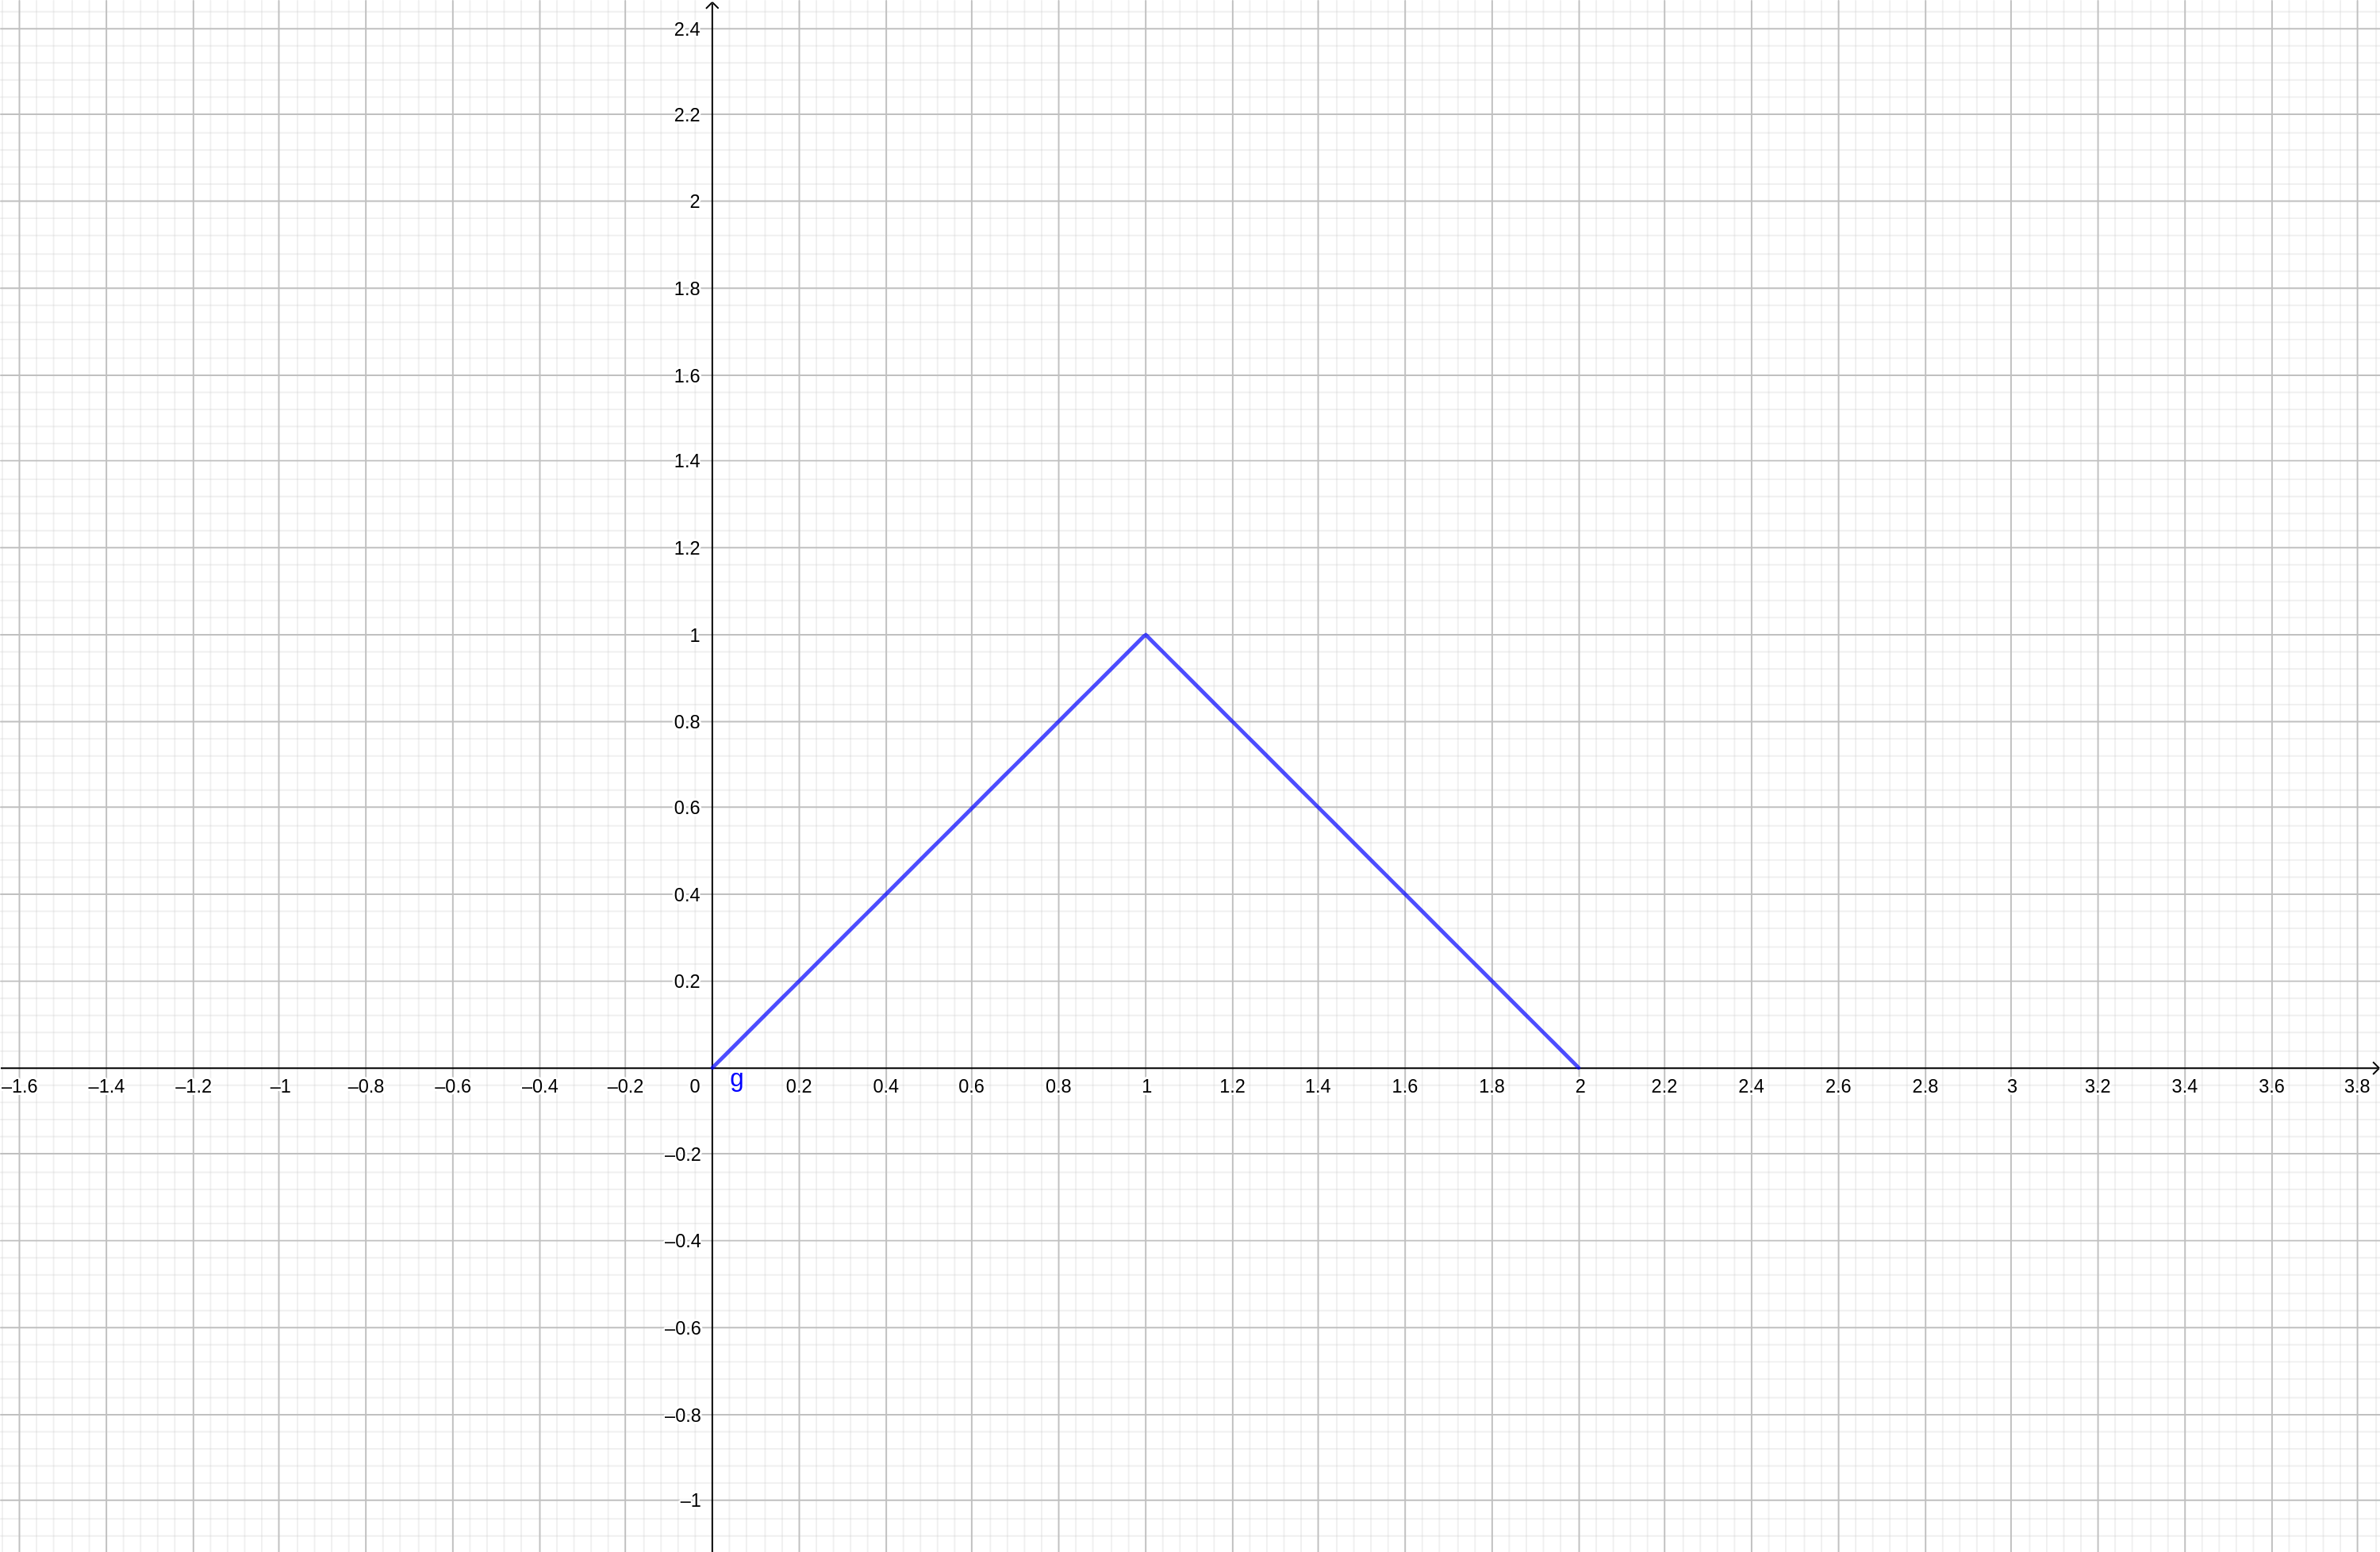
\includegraphics[height=256px]{skizze.png}\\
	c) $[y_0,y_1]\subset [0,1]=\Omega'$ mit $y_0\leq y_1$\\
	\[Y\in[y_0,y_1] = \{x\in\Omega|Y(x)\in[y_0,y_1]\} = \{x\in\Omega| x\in[y_0,y_1]\lor x\in[2-y_1,2-y_0]\}\]
	Das entsteht dadurch, dass wir hier hier beträge haben, also 2 mögliche Fälle beim Auflösen von $Y=1-|X-1|$ nach X bekommen.\\
	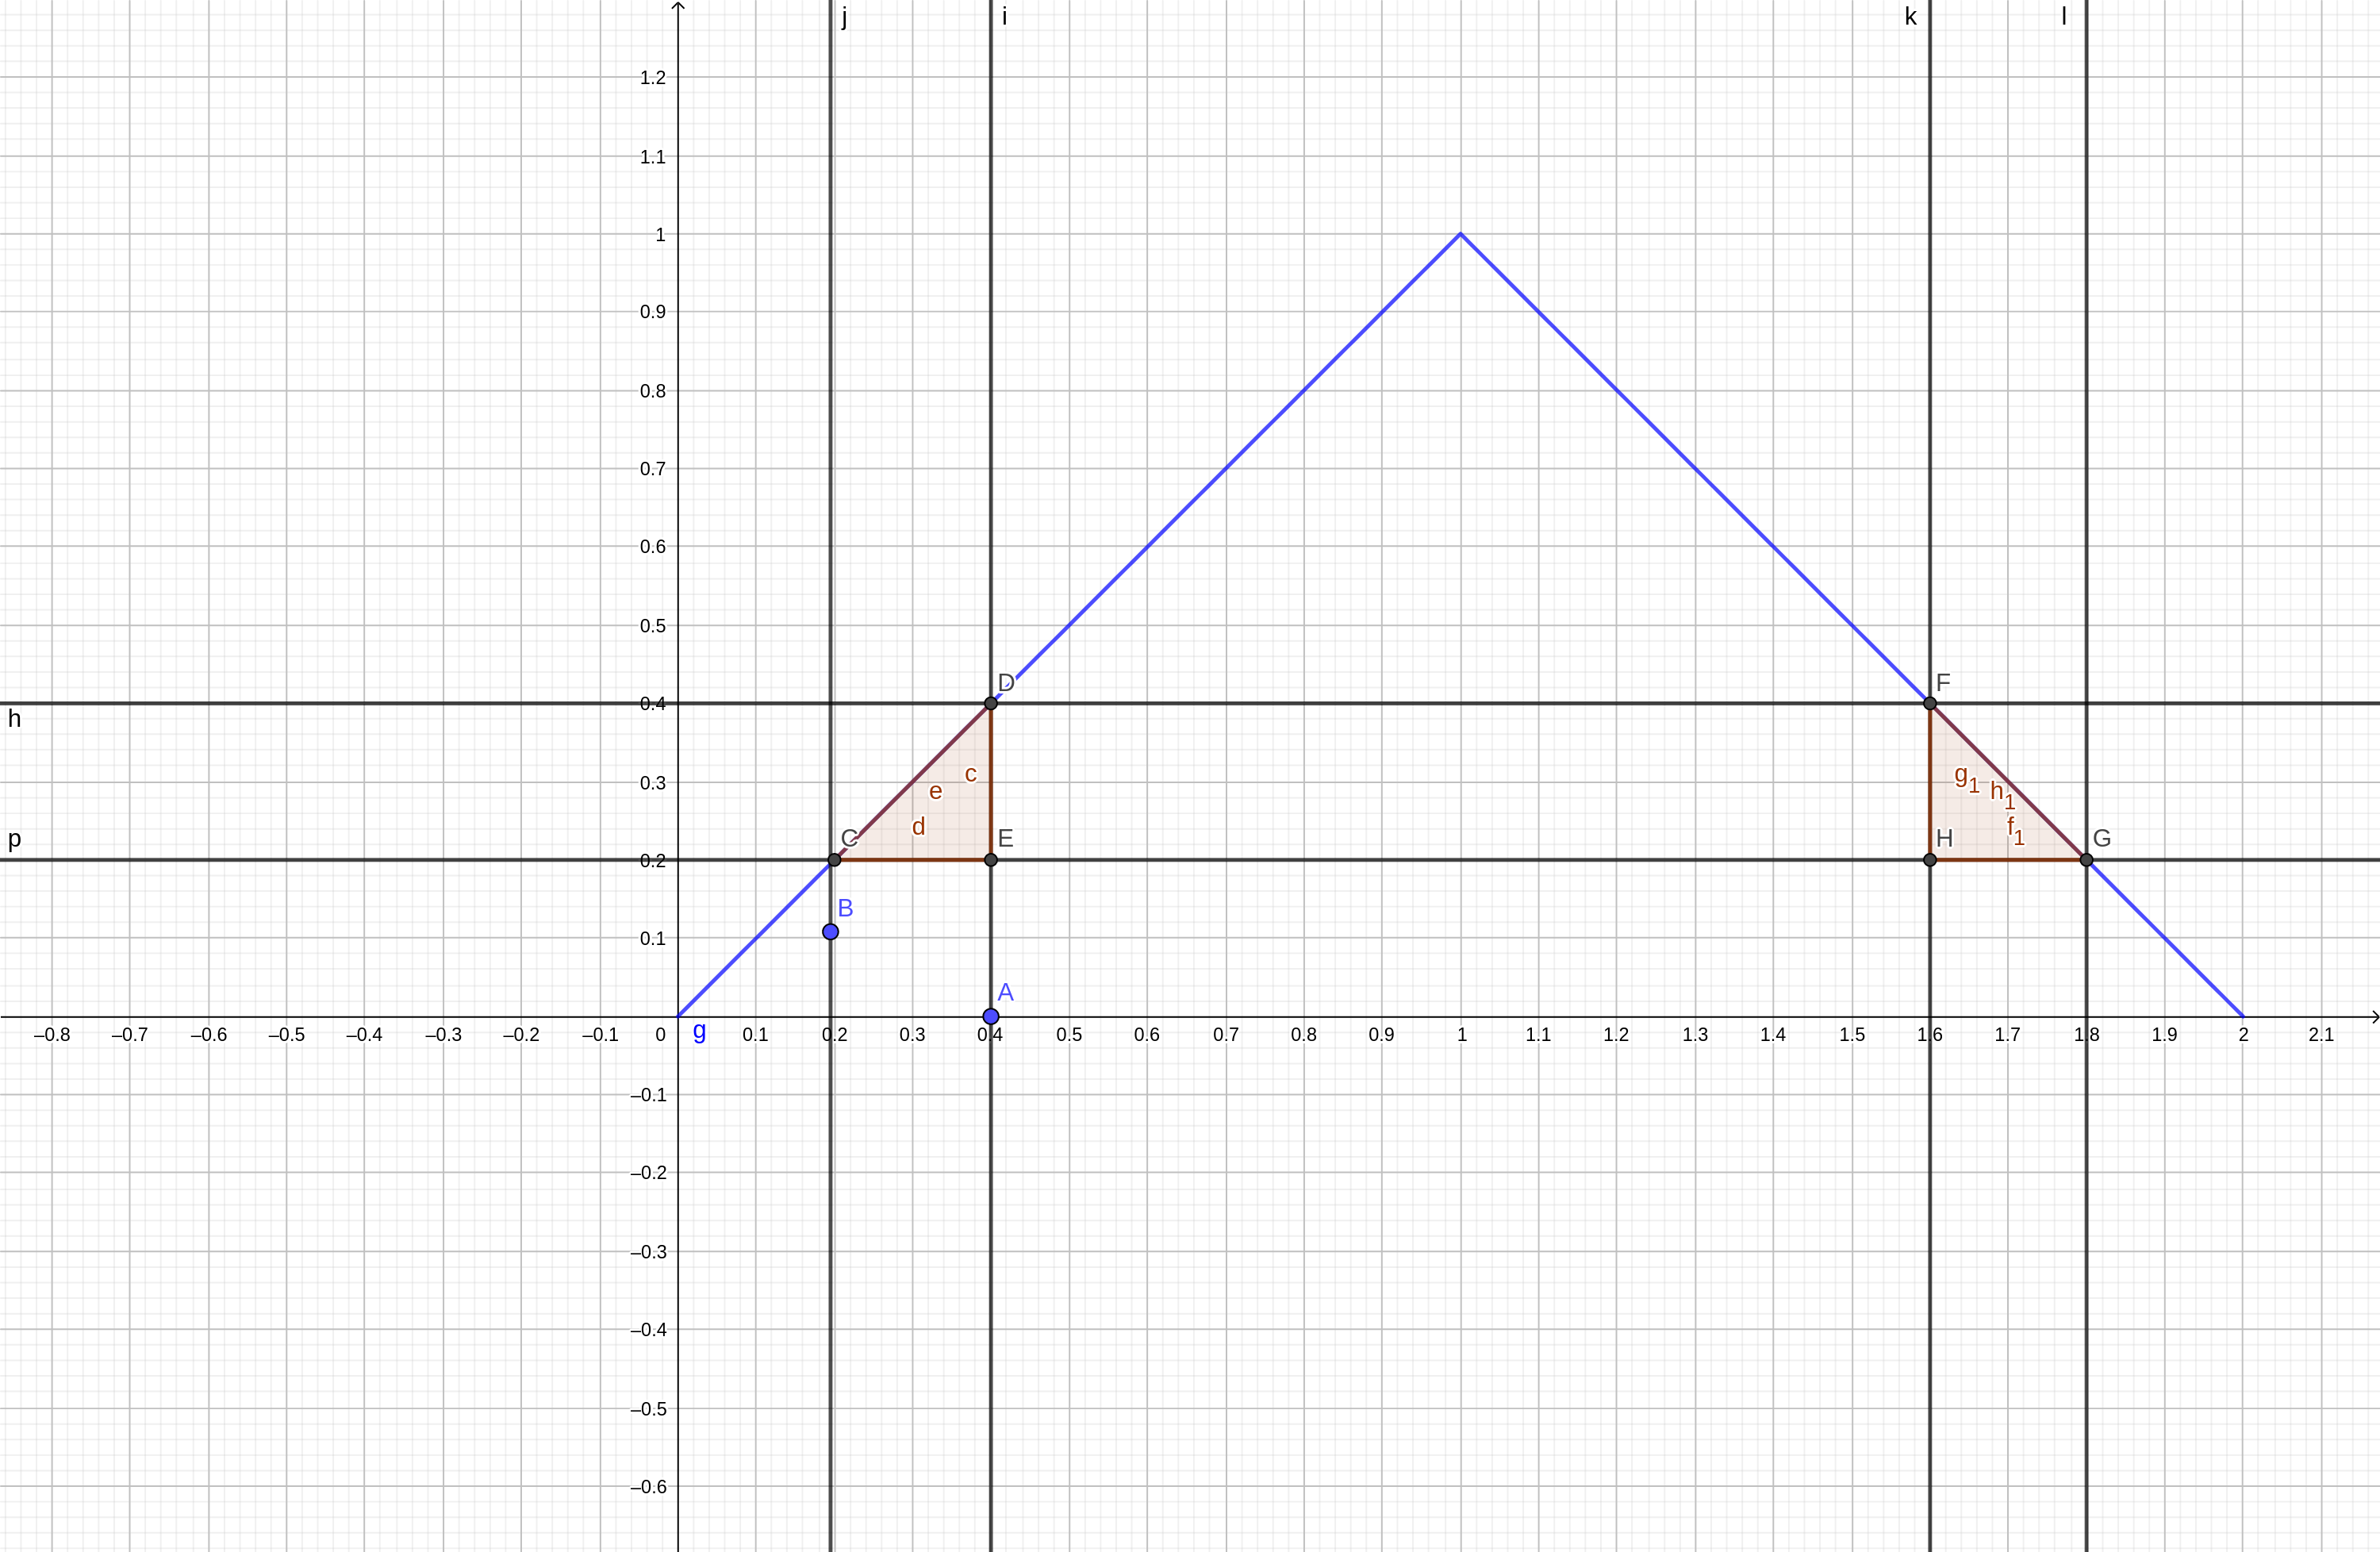
\includegraphics[height=256px]{skizzeIntervalle.png}
	\[P_Y([y_0,y_1]) =P_X([y_0,y_1])+P_X([2-y_1,2-y_0]) = \frac{2}{3} (y_1-y_0)+\int^{2-y_0}_{2-y_1}f(x) dx\]
	\[= \frac{2}{3} (y_1-y_0)+\frac{2}{3}[min(2-y_0,1.5)-min(2-y_1,1.5)]\]
	\[=\begin{cases}\frac{2}{3} (y_1-y_0)& 2-y_1\geq \frac{3}{2}\\
	\frac{2}{3} (y_1-y_0)+\frac{2}{3}(1.5-(2-y_1)& 2-y_1\leq 1.5 \land 2-y_0\geq 1.5\\
	\frac{2}{3} (y_1-y_0)+\frac{2}{3}((2-y_0)-(2-y_1)& 2-y_1\leq 1.5 \land 2-y_0\leq 1.5
	\end{cases}\]
	Es gilt
	\[P(x\leq a)=\frac{d}{dx}\int^{\infty}_{-\infty} f(x)dx=f(x)\]
	\[f_Y(y) = \frac{d}{dy}P((-\infty,y)) = \frac{d}{dy}P([0,1])\]
	Also oben einfach den Integral von $-\infty$ nach y berechnen.\\
	Fall 1:\\
	$y\in[0,1]$ Also nicht nach $-\infty$ gehen, sondern nur bis 0 (darunter ändert sich nichts mehr).\\
	\[\frac{d}{dy} \begin{cases}\frac{2}{3} y\\ \frac{2}{3}y+\frac{2}{3}(y-0.5)\\ \frac{4}{3}y\end{cases}\]
	\[\begin{cases}\frac{2}{3}\\ \frac{2}{3}+\frac{2}{3}\\ \frac{4}{3}\end{cases}\]
	Fall 2: $y\notin [0,1]$\\
	$f_Y(y)=0$\\
	\section{46}
	\[f^{(X;Y)} (x,y)=\frac{x+y}{32}1_{\{1,2\}}(x)1_{\{1,2,3,4\}}(y)\]
	\[f_x^x:= \sum^4_{y=1}f^{(X;Y)}_{(x,y)} = \sum^4_{y=1} \frac{x+y}{32} = \frac{2x+5}{16}\]
	\[f_y^Y:= \sum^2_{x=1}f^{(X;Y)}_{(x,y)} = \sum^2_{x=1} \frac{x+y}{32} = \frac{2y+3}{32}\]
	Also $f_X^X=\frac{2x+5}{16}1_{\{1,2\}}$ $f^Y_Y = \frac{2y+3}{32}1_{\{1,2\}}$\\
	$P(X\geq Y) = \underbrace{P(X=2,Y=1)}_{Sonst\ gilt\ ungleichung\ nicht} = f^{(X;Y)} (2,1) = \frac{2+1}{32} = \frac{3}{32}$\\
	$P(Y\geq 2x)=P(X=1,Y=3)+P(x=1, Y=4) = \frac{4+5}{32}=\frac{9}{32}$
	$P(X+Y=3)= P(X=1,Y=2)+P(X=2,Y=1) = \frac{6}{32}$\\
	c)\\
	Nein: $f_X^X\cdot f_Y^Y=\frac{4x+10}{32}\frac{2y+3}{32} \neq f^{(X;Y)} (x,y)$\\
	Also stochastisch \underline{abhängig}!\\
	Das kann man auch aus dem $P(X+Y=3)$ sehen: Wenn man X=1 wählt, ist man gezwungen Y=2 zu wählen. Somit erzwingt die Wahl von X die Wahl von Y, also stochastisch abhängig!
\end{document}